\begin{figure}[H]
		\begin{center}
			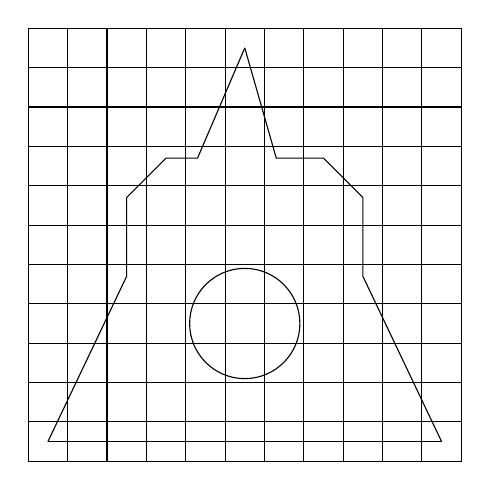
\begin{tikzpicture}[box/.style={rectangle,draw=black, minimum size=0.5cm}]
				\foreach \x in {0,0.5,...,5}
					\foreach \y in {0,0.5,...,5}
						\node[box] at (\x,\y){};
			
				\draw (0, 0) -- (5, 0);
				\draw (0, 0) -- (1.0, 2.1) -- (1.0, 3.1) -- (1.5, 3.6) -- (1.9, 3.6) -- (2.5, 5);
				\draw (5, 0) -- (4.0, 2.1) -- (4.0, 3.1) -- (3.5, 3.6) -- (2.9, 3.6) -- (2.5, 5);
				\draw (2.5, 1.5) circle (0.7);
			\end{tikzpicture}
		\end{center}
		\caption{Наложение многоугольника на растровую матрицу}
		\label{fig_on_rastr}
	\end{figure}